\documentclass[a4paper,11pt,oneside]{book}
\usepackage[utf8]{inputenc}
\usepackage{graphicx}
\usepackage[brazilian]{babel}
\usepackage[hmargin=2cm,vmargin=3.5cm,bmargin=2cm]{geometry}

\setcounter{secnumdepth}{3}		% Add level 3 of sections (can use \subsubsection in books)

\begin{document}

\author{Gustavo Müller Nunes}
\title{Reconhecimento de imagens de gestos e poses de mão em um ambiente automotivo}
\date{January 2014}

\maketitle
\tableofcontents 	%Índice de conteúdos
\listoftables 		%Lista de tabelas
\listoffigures 		%Lista de figuras

\chapter{Objetivo}

O objetivo do trabalho é discutir as principais técnicas para reconhecimento de gestos e poses de mão em um ambiente automotivo.
Os algoritmos e metodologias hoje utilizados para de segmentar e extrair características de imagens e vídeos devem ser estudados e verificados se atingem seu propósito em um ambiente automotivo. Esse ambiente apresenta uma forte variação de luz e ausência de controle nas características da mão e do braço do motorista (cor de pele, braço com ou sem vestimentas e vestimentas de cores e estampas diferentes). As características extraídas são utilizadas como entrada em um classificador responsável por reconhecer gestos e poses de mão, e assim, permitir uma interação com o veículo traduzindo os gestos em comandos para o carro.

\todo{Tradução do artigo \cite{ref2}}

Reconhecimento de gestos baseado em visão é um assunto bastante popular e pesquisado. A busca por mecanismos que tornem a interação entre homem e máquina mais intuitiva e natural é constante e vem aumentando com o lançamento de plataformas que auxiliam os desenvolvedores nos complexos algoritmos que envolvem essa área.
O lançamento do Kinect, da Microsoft \cite{kinect}, e da plataforma de desenvolvimento da Intel, chamada Intel Perceptual Computing \cite{intel} (ambas com câmeras de profundidade) vem popularizando o desenvolvimento de aplicativos e revolucionando o jeito que interagimos com os jogos e computadores. 

\begin{figure}[ht!]
\centering
\fbox{
  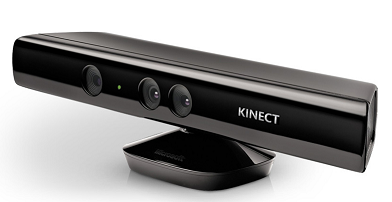
\includegraphics[width=0.3\textwidth]{image/kinect_camera.png}
  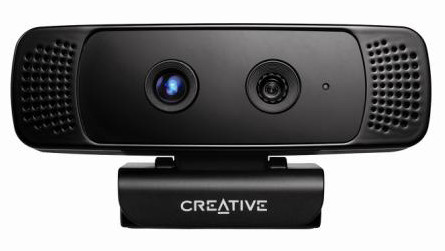
\includegraphics[width=0.3\textwidth]{image/intel_creative_camera.jpg}}
  \caption{Kinect, da Microsoft, e a câmera da \textit{Creative} com parceria da Intel}
  \label{fig:depth_camera}
\end{figure}

O uso de câmeras em carros e caminhões também tem aumentando nos últimos anos. Sistemas de segurança capazes de verificar se o motorista esta saindo indevidamente da faixa, ou se o veículo esta em rota de colisão com algum outro automóvel ou objeto e até mesmo monitorando o stress do motorista já são comuns em vários modelos de veículos. Mas pouco vimos o uso dessas câmeras para interação do motorista com a grande quantidade de controles de temos no carro.




\chapter{Teoria}
\section{Momentos}

Momentos são medições escalares usadas para caracterizar uma função e capturar suas características mais significativas. São bastante usados a centenas de anos em estatística para descrever a forma de uma função de densidade probabilística e em corpos rígidos para medir a distribuição de massa.
Do ponto de vista matemático, momentos são "projeções" de uma função em uma base polinomial (da mesma forma que, transformada de Fourier é uma projeção em uma base de funções harmônicas).

Definindo então uma imagem como sendo uma função real \( f(x,y) \) de duas variáveis em a compact support \( D \subset \mathbb{R} \subset \mathbb{R} \) e tento uma integral finita diferente de zero. Podemos definir o momento de forma genérica \( M_{pq}^{(f)} \) de uma imagem \( f(x, y) \), onde \( p, q \) são valores não negativos e inteiros e \( r = p + q \) é a ordem do momento, como:

\[ M_{pq}^{(f)} = \iint_D p_{pq} (x, y) f(x, y) \,dx \,dy \]

\section{Momentos invariantes em translação, rotação e escala}

\subsection{Introdução}

Translação, rotação e escala (abreviado como TRS, do inglês \textit{Translation, rotation and scaling}) são as transformações de coordenadas espacial mais simples. TRS é uma transformada de 4 parâmetros, que pode ser descrita como

\[x' = sR \cdot x + t \]

\todo{Verificar link. \\
http://docs.opencv.org/doc/tutorials/imgproc/shapedescriptors/moments/moments.html}


\begin{thebibliography}{2}
 
\bibitem{ref1} Alberto Simões ,{\em Uma não tão pequena introdução ao \LaTeX},2007.
\bibitem{ref2} Autor do livro ,{\em Título do Livro}, Ano de edição,Editora,etc.
 
\end{thebibliography}

\end{document}